\documentclass[12pt]{article}

\usepackage{graphicx}

\title{EECS 440 PA1 Writeup}
\author{Andrew Mason}

\begin{document}
\maketitle

\begin{enumerate}
  \item What is the accuracy of the classifier on each dataset when the depth
    is set to 1? (i.e. the tree has just one test)
    \begin{enumerate}
      \item Voting: 56.1\%
      \item Volcanoes: 32.8\%
      \item Spam: 62.5\%
    \end{enumerate}
  \item
    \begin{enumerate}
      \item Voting: "Iran Threat Reduction Act of 2011"\\
        This makes sense as a "good" first test to me. Iran seems to be a
        particular polarizing and partisan issue, so it should divide the
        examples pretty well into R/D buckets.
      \item Spam: "geoDistance"\\
        This also makes sense as a good first test. When you are communicating
        over the internet, often you communicate with those around you (i.e.
        emailing your professor for help on a programming assignment), so it
        seems intuitive to say that the further away geographically two parties
        are, the more likely the communication is not authentic.
    \end{enumerate}
  \item ~\\
    \begin{tabular}{|r|c|c|}
      \hline
      Depth & Volcano Accuracy & Spam Accuracy \\ \hline
      1 & 32.8\% & 62.5\% \\ \hline
      2 & 32.8\% & 62.5\% \\ \hline
      3 & 32.8\% & 62.5\% \\ \hline
      4 & 32.8\% & 62.5\% \\ \hline
      5 & 32.8\% & 62.5\% \\ \hline
    \end{tabular}

    \begin{figure}
      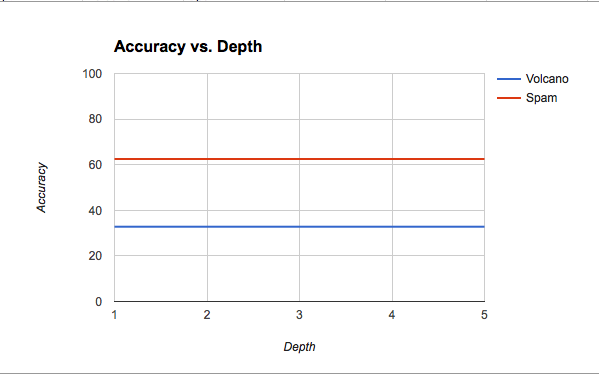
\includegraphics[width=\linewidth]{graph.png}
      \caption{Plot of Accuracy vs. Depth}
    \end{figure}
  \item
    Other observations:\\
    \begin{enumerate}
      \item Increasing depth for the volcano or spam dataset did not seem too
      help much. The average size of the learned tree was always one more than
      the average depth, which means it was basically creating a linked list of
      tests, rather than a well-balanced tree which nicely partitions the
      examples.\\

      I believe this is why the accuracy did not increase with depth.\\
      Note that I did not observe this behavior on the voting dataset, which
      had accuracy increase with depth, and yielded much higher density trees
      (for example, on depth=5, the average tree contained 32.2 nodes, whereas
      for the volcanoe dataset, the average tree at the same depth contained
      only 6 nodes). So, it is possible that the addition of continuous
      attributes (or perhaps the sheer increase in the number of examples) made
      the tree much harder to learn well.
    \end{enumerate}
\end{enumerate}
\end{document}
